\section{Analysis}
Given that all angles in this study are measured in degrees, 
it is essential to convert them into radians for the purposes of 
trigonometric calculations. 
This conversion is achieved using the following formula:
\begin{equation}
    \theta_{\text{rad}} = \frac{2\pi}{\SI{360}{\degree}} \cdot \theta_{\text{deg}},
\end{equation}
where $\theta_\text{deg}$ represents the angle in degrees and 
$\theta_\text{rad}$ denotes the angle in radians.

\subsection{Determination of the Contrast in dependency of the polarisation angle}

As described in Section \ref{sec:contrast}, the minimum 
and maximum intensities for different polarization angles 
are measured. The measured values are listed in Table 
\ref{tab:contrast}.

These values are used to calculate the contrast $K$ for 
both sets of measurements using Equation \eqref{eqn:contrast}. 
Subsequently, the mean and the standard deviation of $K$ are 
computed using \textit{numpy} \cite{numpy}. Figure 
\ref{fig:contrast} visualizes these values of $K$.
\\
For the fit, the function described in Equation 
\eqref{eqn:contrast2} is modified by introducing a constant 
offset angle $\delta$ and a factor $K_0$ which represents the 
maximal contrast. Both parameters are allowed to vary in the 
fit to compensate for deviations between the experimental setup 
and the theoretical model. The resulting function is 
\begin{equation}
    K = 2 K_0|\sin{(\phi-\delta)}\cos{(\phi-\delta)}|
    \label{eqn:K_ana}
\end{equation}
The fit, conducted using \textit{scipy} \cite{scipy}, is displayed 
in Figure \ref{fig:contrast}. The values of the parameters are 
\begin{align*}
    K_0=\num{0.895\pm 0.015} \quad\text{and}\quad \delta=\SI{2.27\pm0.33}{\degree}.
\end{align*}

\begin{figure}[H]
    \centering 
    \includegraphics[width=0.8\textwidth]{build/contrast.pdf}
    \caption{Averaged contrast $K$ as a function of the polarization angle $\phi$ with a fit using the function described in Equation \eqref{eqn:K_ana}.}
    \label{fig:contrast}
\end{figure}

The maximum contrast was measured at a polarization angle of 
$\phi = \SI{130}{\degree}$. Henceforth, the polarization angle 
is set to this value for subsequent measurements.

\begin{table}
    \centering
    \begin{tabular}{S S S S S}
        \toprule
        {$\phi/\si{\degree}$} & {$I_\text{min1}/\si{\volt}$} & {$I_\text{max1}/\si{\volt}$} & {$I_\text{min2}/\si{\volt}$} & {$I_\text{max2}/\si{\volt}$}\\
        \midrule
        0   &  2.02 & 1.75 & 2.12 & 1.80 \\
        5   &  1.82 & 1.55 & 1.92 & 1.53 \\
        10  &  1.82 & 1.26 & 1.87 & 1.23 \\
        15  &  1.91 & 0.99 & 1.88 & 0.95 \\
        20  &  1.73 & 0.74 & 1.78 & 0.69 \\
        25  &  1.64 & 0.52 & 1.63 & 0.51 \\
        30  &  1.59 & 0.33 & 1.56 & 0.43 \\
        35  &  1.51 & 0.27 & 1.51 & 0.31 \\
        40  &  1.55 & 0.22 & 1.61 & 0.25 \\
        45  &  1.61 & 0.18 & 1.51 & 0.20 \\
        50  &  1.73 & 0.16 & 1.76 & 0.18 \\
        55  &  1.88 & 0.15 & 1.94 & 0.17 \\
        60  &  2.05 & 0.19 & 2.10 & 0.20 \\
        65  &  2.26 & 0.28 & 2.31 & 0.26 \\
        70  &  2.37 & 0.37 & 2.19 & 0.41 \\
        75  &  2.34 & 0.60 & 2.31 & 0.56 \\
        80  &  2.50 & 0.86 & 2.38 & 0.88 \\
        85  &  2.47 & 1.37 & 2.45 & 1.22 \\
        90  &  2.31 & 1.77 & 2.25 & 1.62 \\
        95  &  2.65 & 1.79 & 2.58 & 1.77 \\
        100 &  3.23 & 1.54 & 3.27 & 1.53 \\
        105 &  3.77 & 1.28 & 3.68 & 1.32 \\
        110 &  4.12 & 1.06 & 4.13 & 1.03 \\
        115 &  4.50 & 0.72 & 4.63 & 0.70 \\
        120 &  5.18 & 0.49 & 5.28 & 0.47 \\
        125 &  5.89 & 0.29 & 5.73 & 0.35 \\
        130 &  6.09 & 0.24 & 6.07 & 0.25 \\
        135 &  5.87 & 0.27 & 6.03 & 0.26 \\
        140 &  5.95 & 0.37 & 5.96 & 0.35 \\
        145 &  5.75 & 0.55 & 5.65 & 0.61 \\
        150 &  5.46 & 0.68 & 5.71 & 0.83 \\
        155 &  5.00 & 0.97 & 5.12 & 1.01 \\
        160 &  4.64 & 1.31 & 4.69 & 1.34 \\
        165 &  3.72 & 1.48 & 3.78 & 1.55 \\
        170 &  3.21 & 1.60 & 3.29 & 1.72 \\
        175 &  2.47 & 1.79 & 2.70 & 1.85 \\
        180 &  2.12 & 1.79 & 2.15 & 1.81 \\
        \bottomrule
    \end{tabular}
    \caption{Measured minimal and maximal intensity for different polarisation angles $\phi$.}
    \label{tab:contrast}
\end{table}

\subsection{Determination of the Refractive Index of Glass}
For the measurement of the refractive index, two glass plates 
are placed into the beams of the interferometer as described 
in Section \ref{sec:measurement_glass}. Since the glass plates 
are tilted by $\theta_0 = \pm \SI{10}{\degree}$, Equation 
\eqref{eqn:delta} can be simplified with $\theta_1 = -\theta_2 = \SI{10}{\degree}$ to  
\begin{equation}
    \Delta\Phi(\theta)=2\pi\frac{D}{\lambda_\text{vac}}\frac{n-1}{n}\cdot 2\theta_0\theta.
\end{equation}
This, combined with the relation \eqref{eqn:M}, results in 
\begin{equation}
    M=\frac{D}{\lambda_\text{vac}}\frac{n-1}{n}\cdot 2\theta_0\theta
    \label{eqn:M_ana}
\end{equation}
with the wavelength $\lambda = \SI{632.99}{\nano\metre}$ of 
the laser and the thickness $D = \SI{1}{\milli\metre}$ of 
the glass planes. 

Table \ref{tab:glass} shows the measured 
values for $M$ at different angles $\theta$. 
Equation \eqref{eqn:M_ana} is fitted to the average $M$ of 
all measured number of maxima, varying the parameter $n$.
Figure \ref{fig:glass} displays the fit to the mean values of $M$ with the 
standard deviation represented as error bars.
The fit yields a value of  
\begin{equation*}
    n=\SI{1.485 \pm 0.013}{}
\end{equation*}
for the refractive index of the glass plates.

\begin{table}
    \centering
    \sisetup{table-format=2.0}
    \begin{tabular}{S S S S S S S S S S S[table-format=2.1] @{${}\pm{}$} S[table-format=1.1]}
        \toprule
        {$\theta/\si{\degree}$} & {$M_1$} & {$M_2$} & {$M_3$} & {$M_4$} & {$M_5$} & {$M_6$} & {$M_7$} & {$M_8$} & {$M_9$} &  \multicolumn{2}{c}{$M$}\\
        \midrule
        2 & 6  & 5  & 7  & 5  & 7  & 6  & 7  & 8  & 9   & 6.7 & 1.2  \\
        4 & 12 & 9  & 13 & 13 & 13 & 11 & 11 & 15 & 14  & 12.3 & 1.7 \\
        6 & 19 & 15 & 21 & 16 & 20 & 17 & 20 & 22 & 20  & 18.9 & 2.2 \\
        8 & 27 & 16 & 25 & 23 & 24 & 25 & 25 & 26 & 25  & 24.0 & 3.0 \\
        10 & 33 & 22 & 36 & 36 & 33 & 35 & 33 & 34 & 33 & 32.8 & 4.0 \\
        \bottomrule
    \end{tabular}
    \caption{Measured values of the number of maxima $M_i$ that passed the center for different angles $\theta$ and the calculated average $M$ with standard deviation.}
    \label{tab:glass}
\end{table}

\begin{figure}
    \centering 
    \includegraphics[width=0.8\textwidth]{build/n_glass.pdf}
    \caption{Averaged number of maxima $M$ as a function of the angle $\theta$ with a fit using the function described in Equation \eqref{eqn:M_ana}.}
    \label{fig:glass}
\end{figure}

\subsection{Determination of the Refractive Index of Gas}
The measured values for the number of maxima $M$ that passed 
the center for different pressures are listed in Table \ref{tab:gas}. 
Figure \ref{fig:gas} visualizes the averaged values of $M$ as a 
function of the pressure $p$.

In the case where $n \approx \num{1}$, the Lorentz-Lorenz law 
\eqref{eqn:LLL} can be simplified to 
\begin{equation}
    n=\frac{3}{2}\frac{Ap}{RT}+1.
    \label{eqn:n_gas}
\end{equation}
With the measured room temperature $T_{\text{room}} = \SI{21.8}{\celsius}$ 
and $L = \SI{100.0 \pm 0.1}{\milli\metre}$, this results in a linear function 
\begin{equation}
    n(p)=\frac{3}{2}\frac{p}{RT_\text{room}}\cdot a+b
    \label{eqn:M_gas}
\end{equation}
where the parameters $a$ and $b$ are fitted to the data. 
The fit is shown in Figure \ref{fig:gas}. The values of the 
parameters are 
\begin{align*}
    a=\num{4.44 \pm 0.02} \quad\text{and}\quad b=\num{0.9999987 \pm 0.0000008}.
\end{align*}
Plugging these values into Equation \eqref{eqn:n_gas} with a 
temperature of $T = \SI{15}{\degreeCelsius}$ and a pressure of 
$p = \SI{1013}{\hecto\pascal}$ leads to the measured refractive 
index of air at standard atmospheric conditions:
\begin{equation*}
    n_\text{gas}=\SI{1.0002734\pm 0.0000015}.
\end{equation*}

\begin{table}
    \centering
    \begin{tabular}{S S S S S S}
        \toprule
        {$p/\si{\milli\bar}$} & {$M_1$} & {$M_2$} & {$M_3$} & {$M_4$} & {$M_5$}\\
        \midrule
        50   & 2  &  1 &  2 &  2 &  2 \\ 
        100  & 4  &  3 &  4 &  4 &  4 \\ 
        150  & 6  &  6 &  6 &  7 &  7 \\ 
        200  & 9  &  8 &  9 &  9 &  9 \\
        250  & 11 & 10 & 11 & 11 & 11 \\
        300  & 13 & 12 & 13 & 13 & 13 \\
        350  & 15 & 14 & 15 & 15 & 15 \\
        400  & 17 & 16 & 18 & 17 & 17 \\
        450  & 19 & 18 & 20 & 19 & 19 \\
        500  & 21 & 20 & 22 & 21 & 21 \\
        550  & 23 & 22 & 24 & 23 & 23 \\
        600  & 25 & 25 & 26 & 25 & 26 \\
        650  & 28 & 27 & 29 & 28 & 28 \\ 
        700  & 30 & 29 & 31 & 30 & 30 \\ 
        750  & 32 & 31 & 33 & 32 & 32 \\
        800  & 34 & 33 & 35 & 34 & 34 \\
        850  & 36 & 35 & 37 & 36 & 36 \\
        900  & 38 & 37 & 40 & 38 & 38 \\
        950  & 40 & 40 & 43 & 40 & 41 \\
        1000 & 43 & 42 & 45 & 43 & 43 \\
        \bottomrule
    \end{tabular}
    \caption{Measured values of the number of maxima $M$ that passed the center for different gas pressures $p$.}
    \label{tab:gas}
\end{table}

\begin{figure}
    \centering 
    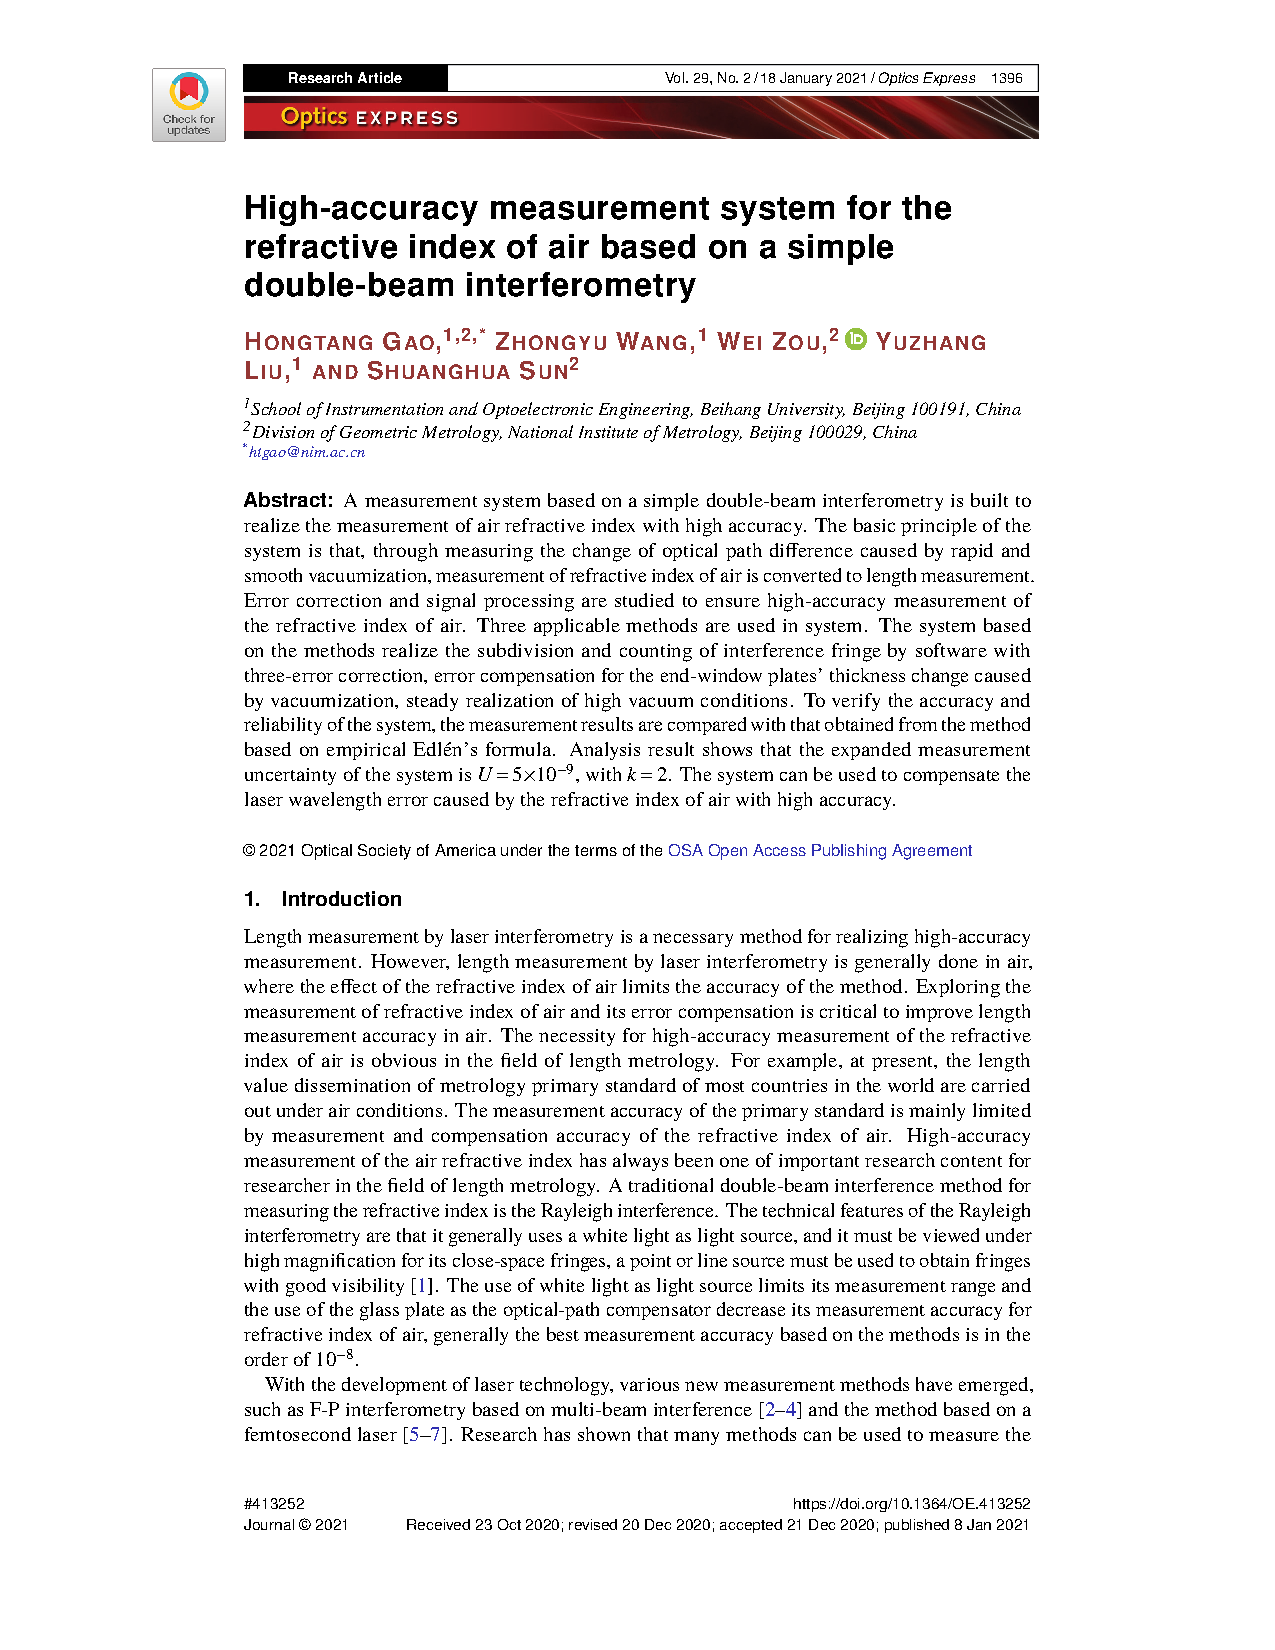
\includegraphics[width=0.8\textwidth]{build/n_air.pdf}
    \caption{Averaged number of maxima $M$ as a function of the gas pressure $p$ with a fit using the function described in Equation \eqref{eqn:M_gas}.}
    \label{fig:gas}
\end{figure}
